\pagebreak
\section{SOP: Pseudonymiziation and survey handling}
\label{section:sop_aliias}

\par\noindent\rule{\textwidth\color{pniblue}}{0.4pt}
\subsection*{Step 1. Start ALIIAS}
\addcontentsline{toc}{subsubsection}{Starting ALIIAS}

To start ALIIAS, \textbf{first insert the hardware key}, then double-click the \path{start_pseudoid} icon (\path{start_pseudoid.exe} or \path{start_pseudoid.bat}, depending on your installation, see section \ref{section:sop_installation}). A new browser page will automatically be opened (with the default web browser of the system).

\small\setlength\fboxsep{5pt}\setlength\fboxrule{1pt}
\fcolorbox{pniblue}{pniblue!5}{\begin{minipage}{0.9\textwidth}
In case of trouble see points \ref{faq:err404}, \ref{faq:nobrowser} and \ref{faq:nostart} in section \ref{section:faq} ("Troubleshooting").
\end{minipage}}

\large

\par\noindent\rule{\textwidth\color{pniblue}}{0.4pt}
\subsection*{Step 2. Log in to activate LimeSurvey integration}
\addcontentsline{toc}{subsubsection}{Log in}

\begin{figure}[H]
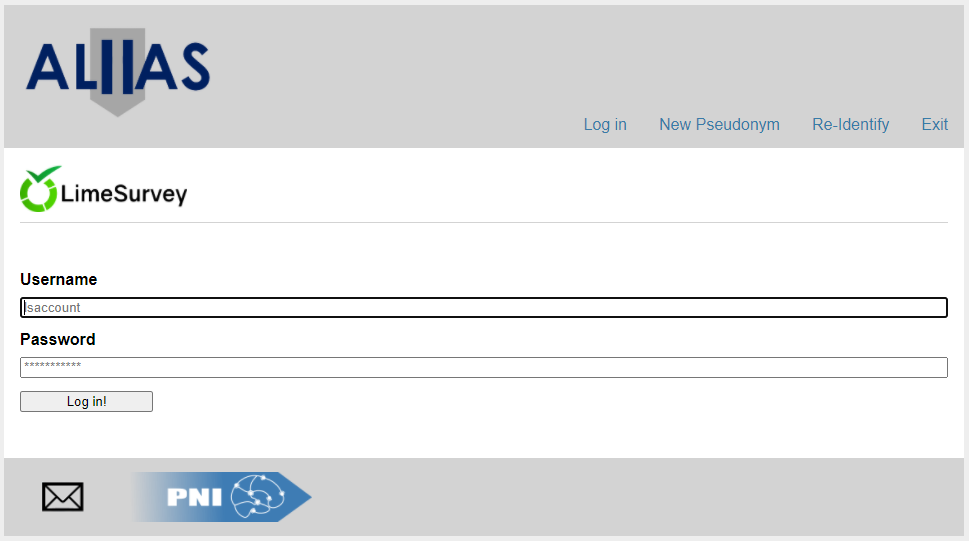
\includegraphics[width=0.9\textwidth]{docs/fig/01_login.PNG}
\end{figure}

After start, ALIIAS lands on the 'Log-in' page.
The header of the page displays the ALIIAS logo and a menu of available pages ('Log in', 'New Pseudonym', 'Re-Identify' and 'Exit'). The footer contains the contact details of the developers.
Stay on the 'Log in' page and provide your LimeSurvey user name and password and click on 'Log in!'.

\small\setlength\fboxsep{5pt}\setlength\fboxrule{1pt}
\fcolorbox{pniblue}{pniblue!5}{\begin{minipage}{0.9\textwidth}
IMPORTANT NOTE: It is possible, but \textbf{not recommended}, to use ALIIAS without logging-in with the LimeSurvey account. The only exception is when internet connection is broken but the researcher must proceed with the experiment. In this case, the researcher is still able to obtain pseudonyms, but the LimeSurvey integration will be not functional and the participant has to be added to the surveys manually.
\end{minipage}}

\small\setlength\fboxsep{5pt}\setlength\fboxrule{1pt}
\fcolorbox{pniblue}{pniblue!5}{\begin{minipage}{0.9\textwidth}
In case of trouble during log in see point \ref{faq:ls_login} in section \ref{section:faq} ("Troubleshooting").
\end{minipage}}
\large

\par\noindent\rule{\textwidth\color{pniblue}}{0.4pt}
\subsection*{Step 3. Enter personal data of the participant}
\addcontentsline{toc}{subsubsection}{Enter Personal Data}

In case of successful log in, user name is displayed in the top menu and, ALIIAS automatically switches to the 'New Pseudonym' page. Enter the following personal details of the participant: first name, family name, place of birth (without country), date of birth, mother's maiden name (family name only). Click on "generate" to create the pseudonym for the given participant.

\begin{figure}[H]
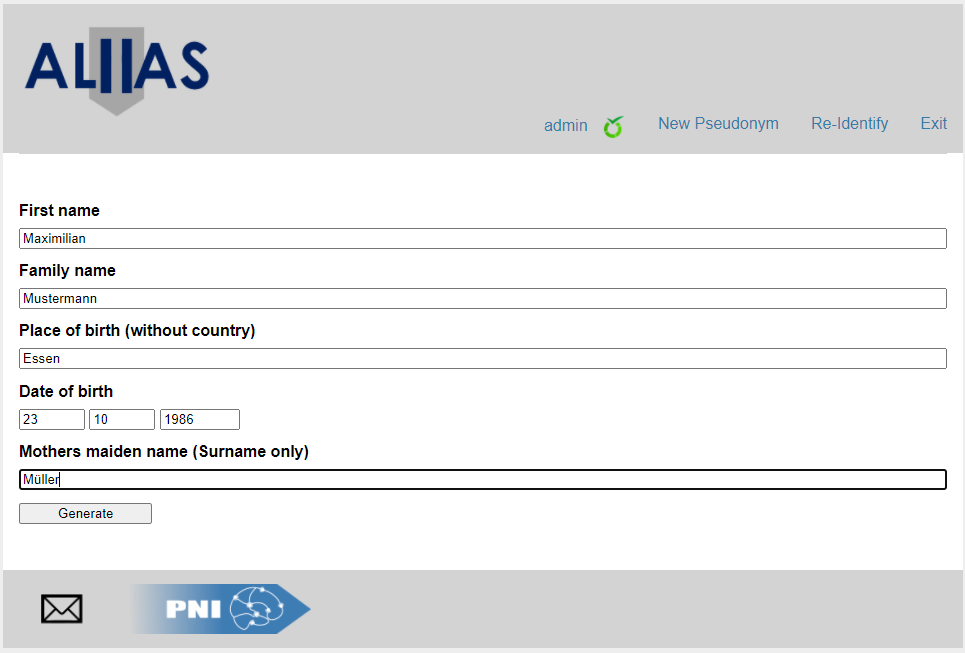
\includegraphics[width=0.6\textwidth]{docs/fig/03_filled.PNG}
\end{figure}

\par\noindent\rule{\textwidth\color{pniblue}}{0.4pt}
\subsection*{Step 4. Check data integrity}
\addcontentsline{toc}{subsubsection}{Check data integrity}

Before displaying the pseudonyms, ALIIAS displays a 'Preview' page. In the 'Personal Info' panel, please \textbf{carefully check all data for typographical errors}, as any error will result in different (invalid) pseudonym. \textbf{Special attention is needed during 'initial registration'} (see section \ref{section:overview} and QC1 in section \ref{section:qc}). When checking for typos, please consider the automatic conversion of ambiguous characters, as listed in Table \ref{tab:typo}.

\large

In case of typographical error, click 'No! Undo Transaction' at the 'All details are correct?' panel and go back to Step 3. 
If there are no typographical errors, proceed to Step 5 (do not press any buttons yet).

\begin{figure}[H]
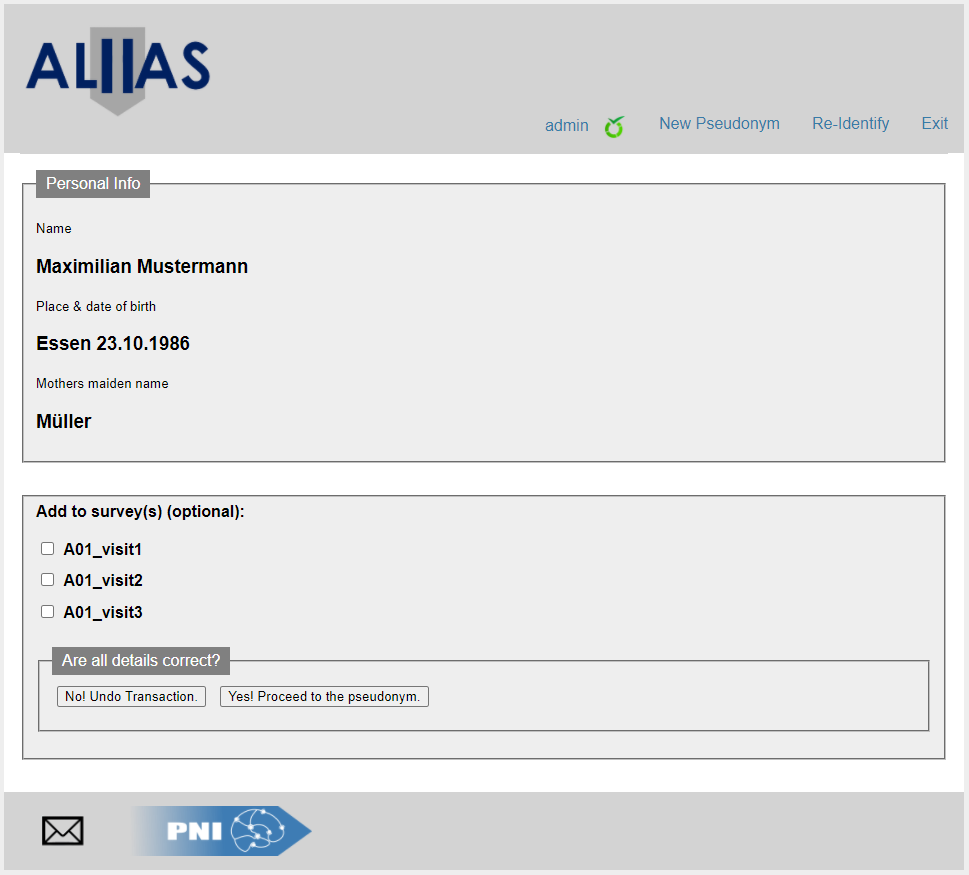
\includegraphics[width=0.8\textwidth]{docs/fig/04_preview.PNG}
\end{figure}

\par\noindent\rule{\textwidth\color{pniblue}}{0.4pt}
\subsection*{Step 5. Survey handling}
\addcontentsline{toc}{subsubsection}{Survey handling}

On the same page, the second panel ('Add to survey(s)') display the status of the present subject in LimeSurvey. Only surveys owned by the current single project are displayed (based on the survey naming conventions in LimeSurvey, see section \ref{section:ls_setup} for more info).

\small\setlength\fboxsep{5pt}\setlength\fboxrule{1pt}
\fcolorbox{pniblue}{pniblue!5}{\begin{minipage}{0.9\textwidth}
Surveys that have already been assigned to the present participant are checked and 'inactive' (i.e. not modifiable). This provides the opportunity for quality-check QC2 (section \ref{section:qc}): At initial registration, the participant is expected not to be assigned to any surveys (as on the presented figure). At repeated measurement points, the participant is expected to be already registered to any surveys preceding the current visit.
\end{minipage}}

\large

If survey information is not consistent with the expectation, double-check personal data and click "No! Undo Transaction" at the bottom.

Otherwise, \textbf{if needed, add the participant to one or more surveys} by ticking the corresponding checkboxes (optional) and click "Yes! Proceed to the pseudonym".

\small\setlength\fboxsep{5pt}\setlength\fboxrule{1pt}
\fcolorbox{pniblue}{pniblue!5}{\begin{minipage}{0.9\textwidth}
It is strongly recommended to add the participant to at least one of the surveys already during the 'initial registration' (section \ref{section:overview}), so that QC2 can be performed at any further pseudonymization sessions.
\end{minipage}}

\large
\par\noindent\rule{\textwidth\color{pniblue}}{0.4pt}
\subsection*{Step 6. Obtaining pseudonym and survey links}
\addcontentsline{toc}{subsubsection}{Obtaining pseudonym and survey links}

On the next page, ALIAS displays information about the updated state of LimeSurvey and lists the surveys to which the participant has been added in the previous step (if any).

Next to the surveys the participant has already been added to, an 'Open Survey' link is displayed. Clicking this link opens the participant-specific survey-url in a new browser page. This url is unique to the participant. Filling in the survey can be started on the present computer, right after finishing the pseudonymization procedure (and exiting ALIIAS) or the URL can be copied (Ctr+V in the address bar) and shared (e.g sent in email) so that the survey participant can open it on another computer (or tablet) or at a later time.

\small\setlength\fboxsep{5pt}\setlength\fboxrule{1pt}
\fcolorbox{pniblue}{pniblue!5}{\begin{minipage}{0.9\textwidth}
In case of trouble when opening the survey link, see point \ref{faq:survey_link} in section \ref{section:faq} ("Troubleshooting").
\end{minipage}}

\large

\begin{figure}[H]
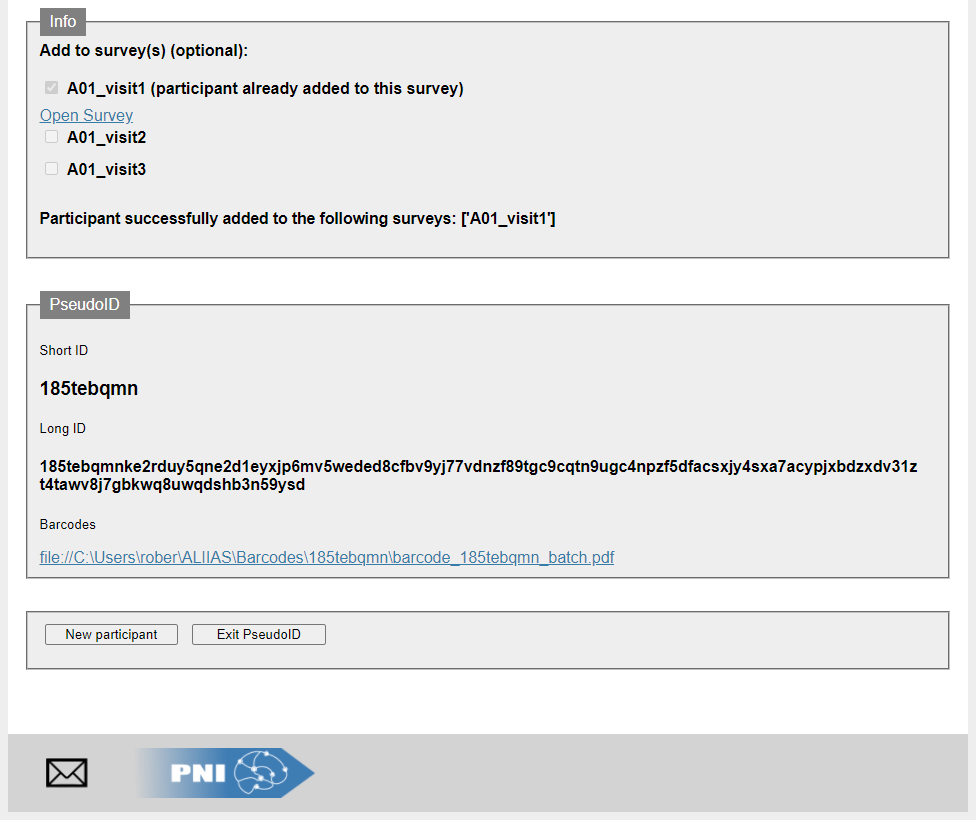
\includegraphics[width=0.9\textwidth]{docs/fig/05_pseudonym.PNG}
\end{figure}

The short and long pseudonyms (or Short ID and Long ID) are displayed at the bottom of the same page, on the 'PseudoID' panel. If the participant has already been added to any of the surveys (displayed on the 'Info' panel), both the short and long IDs are stored in LimeSurvey. 

For behavioral experiments or MRI measurements of this participant, \textbf{the researcher must use the shortID} (9-characters) as participant identifier in the experimental system (e.g. as patient name in the MRI console software).

At the bottom of the page ALIIAS displays the path to the barcodes encoding the short ID. See section \ref{section:sop_barcode} for details on barcode printing.

\par\noindent\rule{\textwidth\color{pniblue}}{0.4pt}
\subsection*{Step 7. Exit ALIIAS}
\addcontentsline{toc}{subsubsection}{Exit ALIIAS}

After obtaining the pseudonym and storing it (automatically in LimeSurvey and/or manually in the dedicated experimental systems), the researcher can generate a new pseudonym in the same ALIIAS-session, by clicking the "New participant" button at the bottom of the page or the "New Pseudonym" menu point in the top menu bar.

If the researcher intends to finish the current ALIIAS session, the "Exit" button at the bottom of the page or the "Exit" menu point in the top menu bar must be clicked.

If the following message is displayed, ALIIAS has exited without any problem. In this case the browser tab can be safely closed.

\begin{figure}[H]
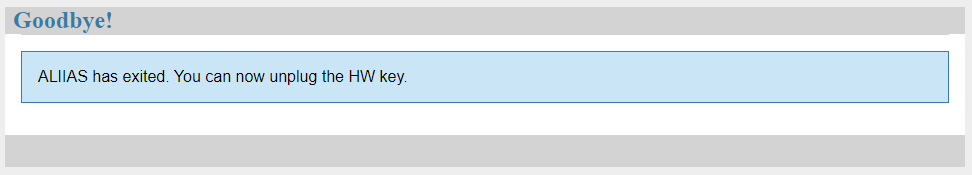
\includegraphics[width=0.9\textwidth]{docs/fig/08_exit.PNG}
\end{figure}

\small\setlength\fboxsep{5pt}\setlength\fboxrule{1pt}
\fcolorbox{pniblue}{pniblue!5}{\begin{minipage}{0.9\textwidth}
IMPORTANT NOTE: closing the browser tab, without exiting ALIIAS is not sufficient! In this case ALIIAS will continue running in the background. This is indicated by the presence of a black command line window. If this happens, see point \ref{faq:exit} in section \ref{section:faq} ("Troubleshooting").
\end{minipage}}
\large
